\section{Einf\"uhrung}
\frame{
	\frametitle{Einführung}
	\vspace{5mm}
	\begin{itemize}
		\item weltweiter Marktanteil: 85 \%
		\vspace{2mm}
		\item Linux-Kernel
		\vspace{2mm}
		\item open source
		\vspace{2mm}
		\item Java (Logik) \& XML (GUI, ressources, config)
	\end{itemize}
}
	% führendes Betriebssystem für Smartphones
	% weltweiter Marktanteil ~85 \%
	% open source
	% Programmierung in Java (Logik) und XML (GUI, ähnlich wie JavaFX, C# mit XAML, etc.)

\frame{
	\frametitle{Versionen}
	\vspace{5mm}
	\begin{itemize}
		\item 2.3 (Gingerbread)
		\vspace{2mm}
		\item 3.0 (Honeycomb)
		\vspace{2mm}
		\item 4.0 (Ice Cream Sandwich)
		\vspace{2mm}
		\item 5.1 (Lollipop) \textrightarrow \ aktuell
	\end{itemize}
}
	% Versionen
	% gut benutzbar seit 2.3.4 (Gingerbread, 2011)
	% seit 3.0 (Honeycomb) Tablet-Support
	% seit 4.0 (Ice Cream Sandwich) viele neue Möglichkeiten, z.B. Fragments
	% --> Seitdem Probleme mit älteren Versionen, Support Libraries
	% aktuell Version 5.1 (Lollipop) --> API-Level 22

\frame{
	\frametitle{Demo-App}
	\begin{columns}[t]
	\column{.7\textwidth}
	\vspace{5mm}
	\begin{block}{Wetter am aktuellen Ort}
		\begin{itemize}
			\item GUI
			\vspace{2mm}
			\item GPS
			\vspace{2mm}
			\item Internet (openweathermap.org)
		\end{itemize}
		\vspace{5mm}
		\( \implies \) reduziert auf Minimal-Anforderungen
	\end{block}

	\column{.3\textwidth}
	\vspace{-1cm}
	\begin{figure}
	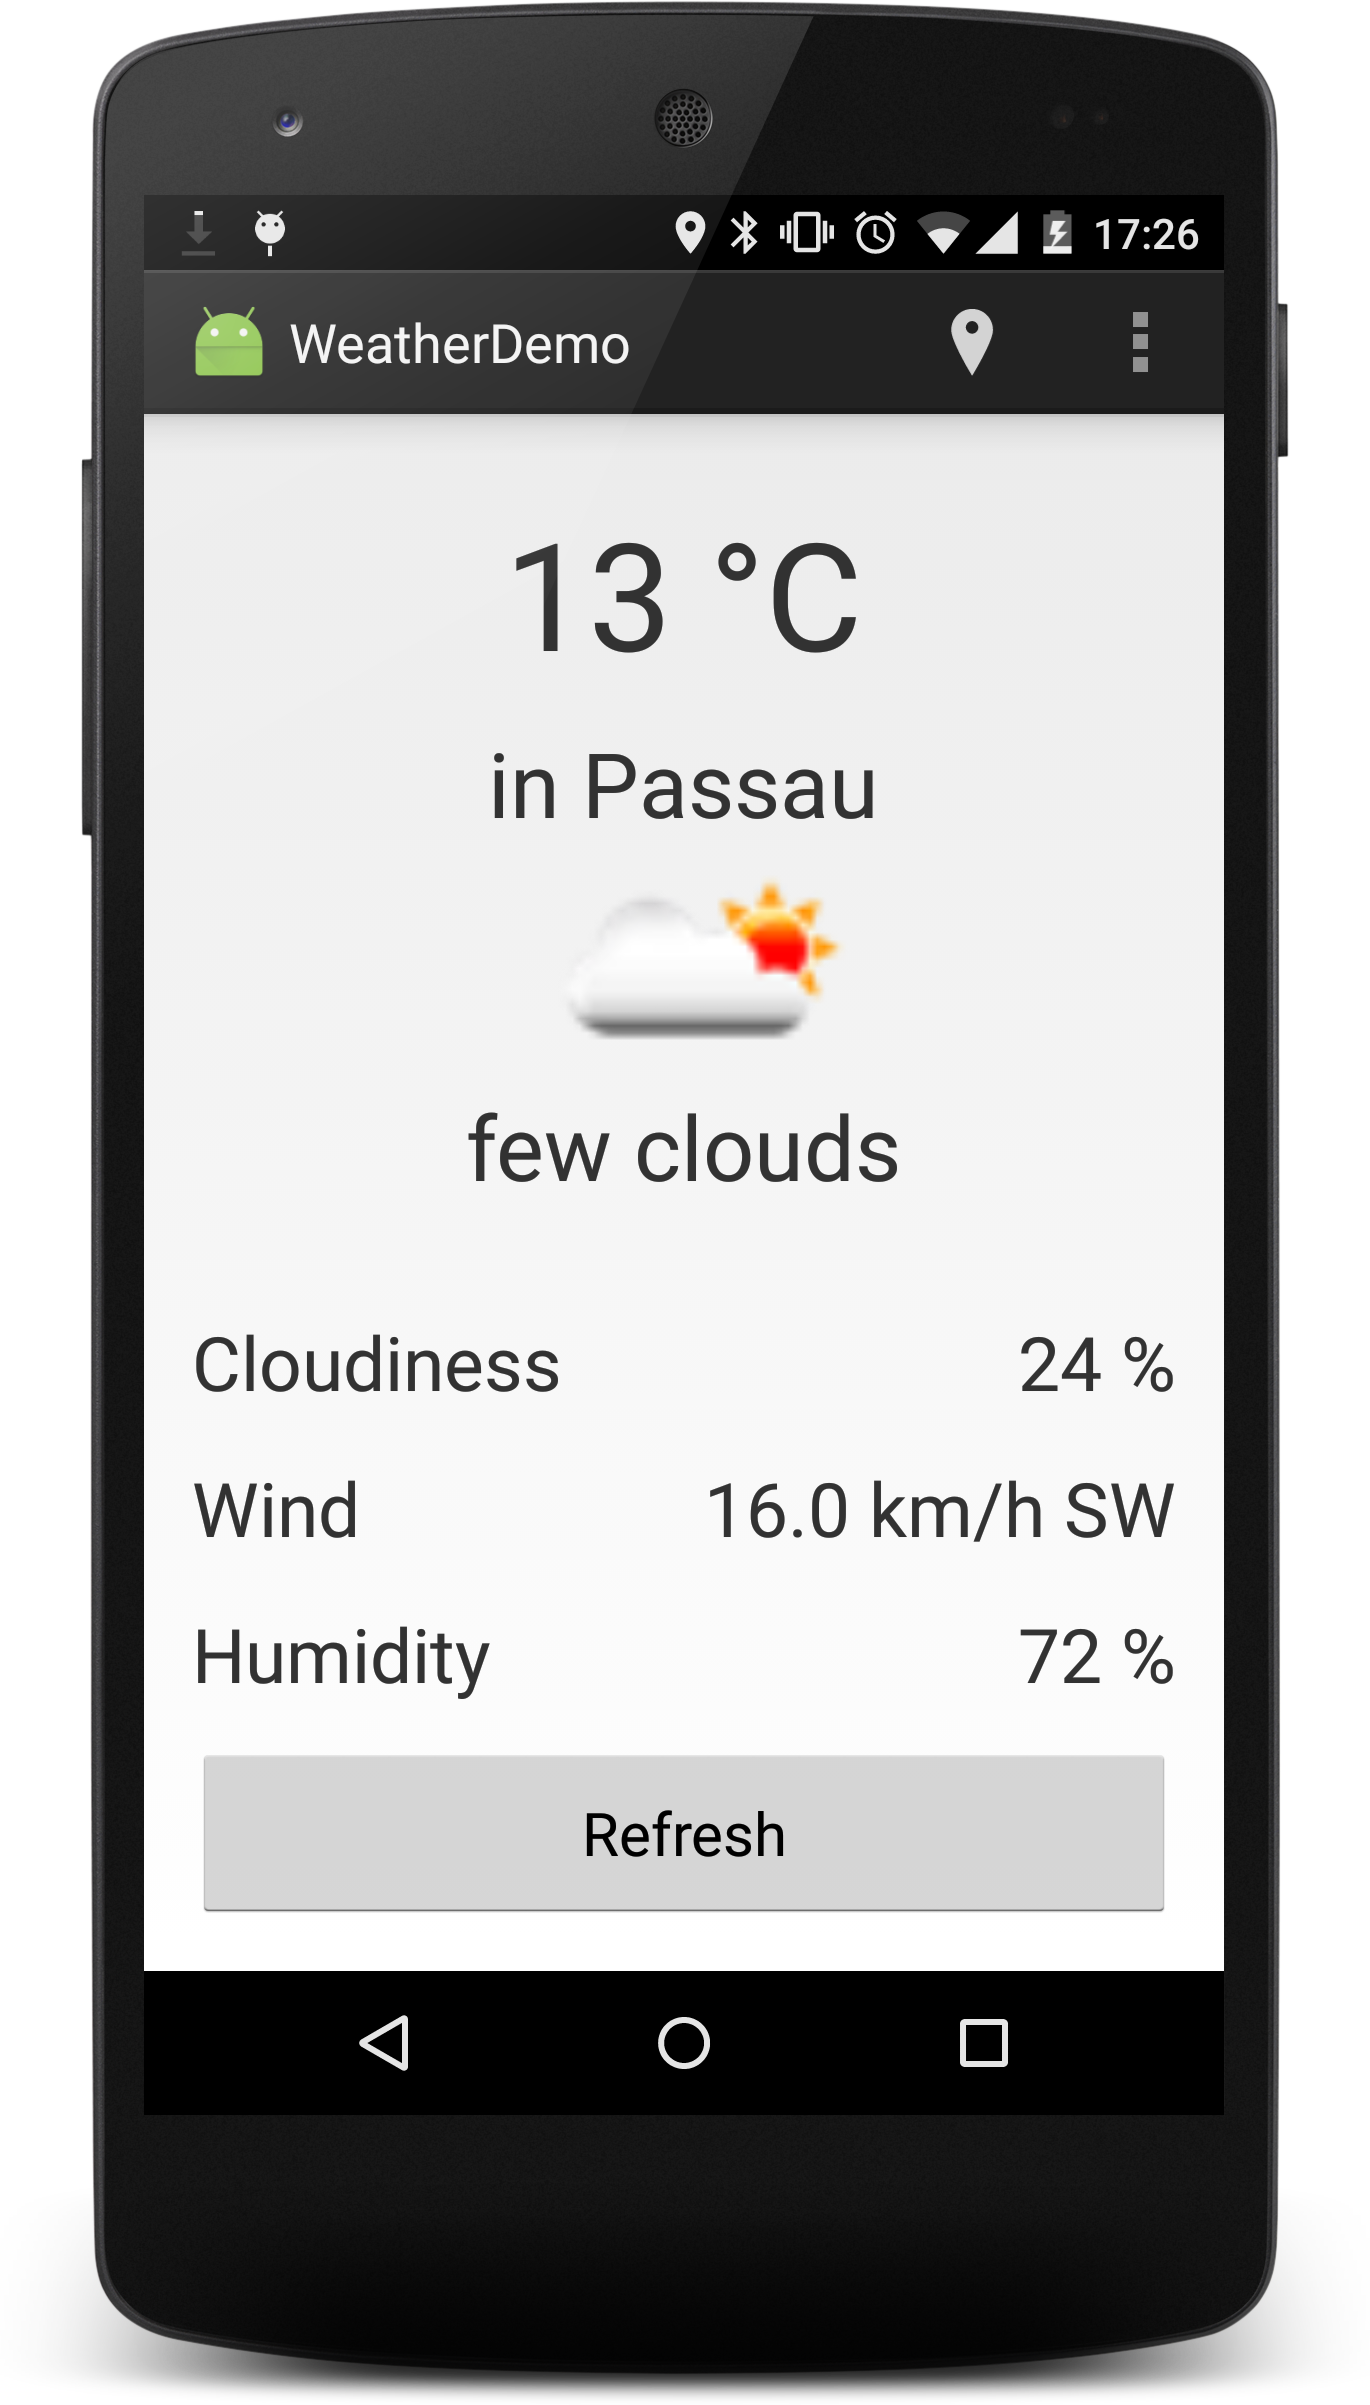
\includegraphics[height=6cm]{pictures/screenshot-main.png}
	\end{figure}
	\end{columns}
}

	% Android als Framework, nicht als Library --> Inversion of control
	% Beispiel-App (reduziert auf Minimal-Anforderungen, ohne (vorerst) unnötigen Ballast), etc.
